\chapter{Relationship between Reading and Functional Network Architecture at Rest}




%% In Task Data
\subsection{Relationship between brain modularity and reading skill}
Original data for the modularity analyses were drawn from the third and fourth waves of a larger longitudinal study (NICHD R01 HD067254, 140 children at first wave). Participants completed out-of-scanner cognitive tests and an in-scanner language task. The fMRI task also included an extensive resting-state baseline in each run, which was the primary target of analysis here. Further information about the aims of this grant can also be found elsewhere \cite{Aboud2016, Wendelken2017}.

\emph{Participants:} Participants were scanned in the summer and fall following completion of third or fourth grade (ages 8-11). All participants met the following criteria: native English speakers; normal hearing; normal or corrected-to-normal vision; no history of major psychiatric illness or traumatic brain injury/epilepsy; and no contraindication to MRI. Participants and their parents gave written consent to participate at the beginning of the study, with procedures carried out in accordance with Vanderbilt University’s Institutional Review Board (IRB). 

Participants completed cognitive tests, including the Wechsler Abbreviated Scale of Intelligence (WASI) \cite{Kaplan1999} and the Test of Word Reading Efficiency (TOWRE) \cite{Torgesen2012}. Demographics and test data are summarized in Table 1. 

\begin{table}
\scriptsize
\renewcommand{\tabcolsep}{0.09cm}
\centering
\begin{tabular}{lc}
\toprule 
 &  Subjects \\ 
\midrule 
Participants & 95 \\ 
Age at Scan & 7.5 (0.5)  \\ 
Gender  &  41 F \\ 
WASI Full-Scale IQ  & 108.5 (16.7) \\ 
TOWRE - Total Word Efficiency & 106.8 (15.8) \\ 
\bottomrule 
\end{tabular}
\caption{Participant demographics.}
\label{table:Ch4_Participants}
\end{table}

\emph{Functional MRI data:} In the MRI scanner, participants performed up to four runs of a language comprehension task, which was crossed on two conditions: the modality of presentation (listening or reading) and the passage genre (expository or narrative).  Each fMRI run had two baseline conditions: a modality-specific baseline task and a resting-state block with a fixation cross. The order and duration for each block varied slightly across runs but was approximately: paragraph 1 (70 s), baseline 1 (70 s), paragraph 2 (70 s), baseline 2 (70 s), and resting-state (270 s). Total scan time was 550 s for all runs, and the average amount of resting-state baseline was 272 s (4 m, 32 s) per run.

A scan run was included in the analysis only if a participant had both listening and reading scans in the same genre (e.g. auditory-expository and reading-expository). Therefore, for each year, a participant had data from either 2 or 4 scan runs (about 9 or 18 minutes of resting-state scan time, respectively). A scan session was excluded based on the following parameters: high-motion volumes exceeding 20 percent; poor task performance; and absence of a paired modality scan. In total, resting-state data from 50 children in the third wave (152 scans) and 45 children in the fourth wave (162 scans) met inclusion criteria. 

\emph{Imaging acquisition and preprocessing: } All fMRI scans were acquired at Vanderbilt University Institute of Imaging Sciences on one of two Philips Achieva 3T MR scanners with a 32-channel head coil. Functional images were acquired using a gradient echo planar imaging sequence with 40 slices acquired parallel to the anterior-posterior commissure plane. Additional imaging parameters for functional images were: 250 dynamics; TR = 2200 ms; TE = 30 ms; FOV = 240*240*120 mm; flip angle = 75 degrees; voxel size = 3 * 3 * 3.2 mm\textsuperscript{3}.

All scans were first preprocessed using a standard pipeline in FSL (version 5.0.9) \cite{Jenkinson2012}, and connectivity analysis was performed in the CONN toolbox \cite{WhitfieldGabrieli2012}. fMRI data were high-pass filtered at 0.008 Hz, motion-corrected, co-registered to a structural image, normalized to MNI space and smoothed by a 5 mm FWHM spherical kernel. Outlier volumes were identified as individual fMRI volumes in which the RMS framewise-displacement exceeded 0.7. fMRI timeseries were corrected using anatCompCorr methods, which uses signal from white matter tissue and cerebrospinal fluid areas to reduce noise not related to brain activity \cite{Chai2012}. Other covariates of no interest included six rigid motion parameters, six derivative motion parameters, and outlier volumes. Finally, we used a weighted general linear model (GLM) to model the resting block and averaged within-subject across scan sessions to get a de-noised resting-state timeseries.

\emph{Network definition:} To build off of previous work, we created networks using 264 nodes originally published by Power and colleagues (2011) \cite{Power2011}. The node set covers the entire brain, including subcortical areas, and has been extensively used in graph theory analyses since its publication (e.g. \cite{Cole2014, Godwin2015, Mattar2015}). Suggested RSN assignments for each node, totaling 13 unique networks, are also available and were used to partition the network into different RSNs. fMRI timeseries correlations were calculated between each of the the 264 nodes, resulting in a single connectivity array for each subject at each time point. Matrices were then thresholded into binary maps at $r$ = 0.15. (To confirm that this particular threshold did not unduly influence results, we also tested thresholds at $r$ = 0.05, 0.10 and 0.20. No significant effect on the results was found.)


\emph{Network analysis:} \textit{Global modularity} ($Q$) quantifies how well the whole-brain network segregates into component RSNs. High modularity indicates that the network has much higher connectivity within RSNs compared to between RSNs; low modularity suggests that nodes do not cluster into RSNs well. For undirected and binary networks, each connection in the array is given a positive value if it links nodes in the same module, and it is then weighted based on the degree of each node and the total network. (For a detailed treatment, see \cite{Rubinov2010}.) Connection-level values were aggregated to get node-by-node and global measures of modularity for each individual, which were then mean-centered and scaled to unit variance. 

A GLM was used to determine the relationship between global modularity and individual performance on the TOWRE (total word efficiency, standard score). If subject data was available at multiple timepoints (n = 30), it was averaged together to produce a single value. Multiple supplementary analyses were also completed to ensure that effects were not driven by cohort or motion confounds: models were also analyzed for Grades 3 and 4 separately, and also when including a measure of subject motion (mean global signal change). We also examined whether there were differences in the modularity relationship between TOWRE subtests (sight word efficiency (SWE) and phonemic decoding efficiency (PDE)).

To test whether there was an RSN-level trend in the modularity-to-reading relationships, node modularity values were also investigated. For the set of nodes comprising each RSN, a one-sample $t$-test was performed to see whether the RSN average was significantly greater than the global node average. 

\emph{Results:} Individual differences in global modularity were predictive of TOWRE - Total Word Efficiency standard scores (Fig. 2A). Modularity had a significant positive relationship with out-of-scanner reading metrics (for all subjects: $r = 0.299$, $p = 0.013$). This effect was also significant when data was analyzed separately by grade ($r_{G3} = 0.333$, $p = 0.014$; $r_{G4} = 0.359$, $p = 0.012$). The two subtests that constitute the TOWRE both showed a positive relationship with global modularity, as well ($r_{PDE} = 0.314$, $p = 0.009$; $r_{SWE} = 0.251$, $p = 0.039$). 

When examined at the individual node level, the average correlation between modularity and TOWRE scores was 0.134. Three RSNs had average node correlations that were significantly higher than this global network mean: the default mode ($r = 0.183$, $p$ \textless $0.001$), visual ($r = 0.183$, $p = 0.004$) and cingulo-opercular networks ($r = 0.224$, $p$ \textless $0.001$) (Fig. 2B). 


\begin{figure}[h!]
\centering
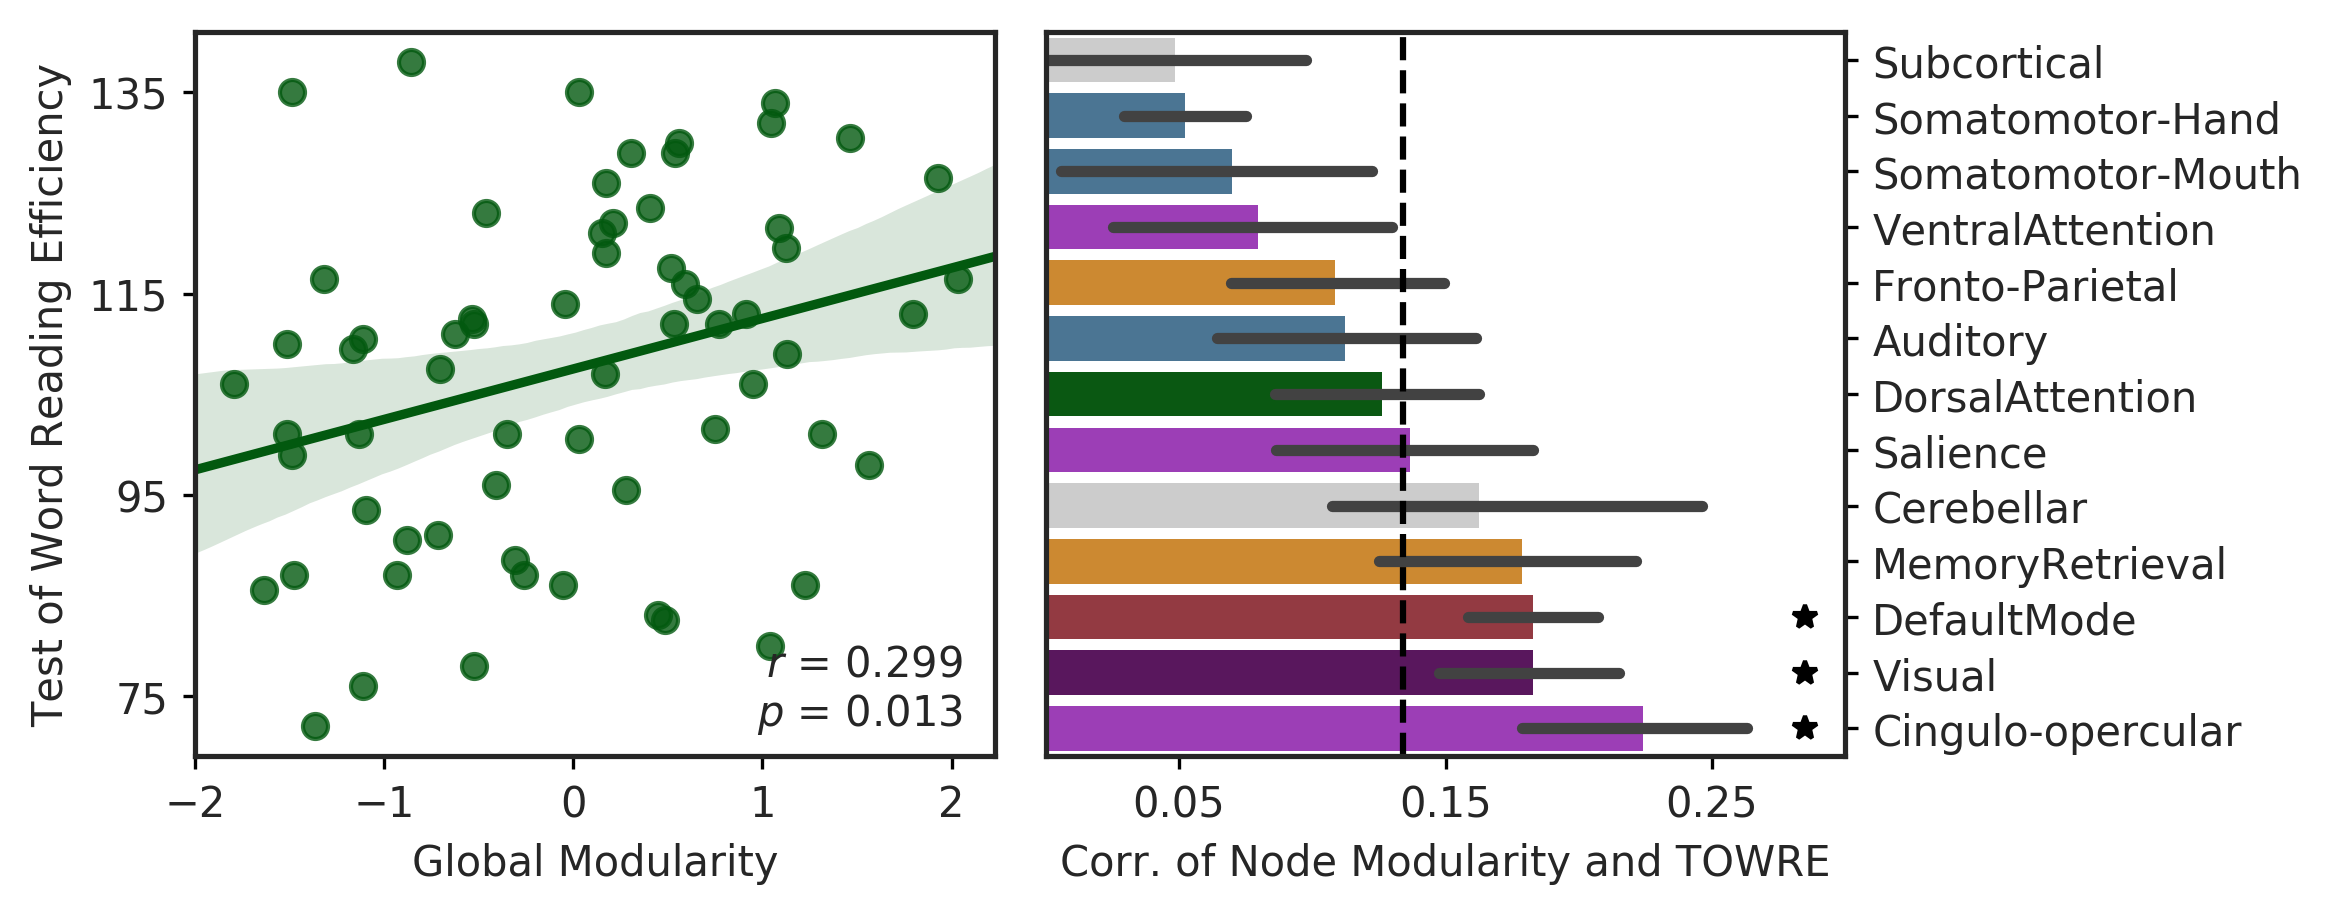
\includegraphics[width=5in]{Ch4_ModularityReading.png}
\caption[Modularity metrics at rest predict reading skill.] {Global modularity, the degree to which a whole-brain network separates into RSNs, was positively related to reading skill across all subjects ($N = 65$). Modularity for individual nodes was also positive overall ($r_{avg} = 0.134$), but was significantly higher for nodes in the visual, default mode and cingulo-opercular RSNs ($p < 0.01$). RSN colors correspond to the dominant Yeo RSN displayed in Fig. 1.}
\label{fig:texlogo}
\end{figure}


